\documentclass[12pt,fleqn]{article}
\usepackage[margin=1in,top=1in,bottom=1in]{geometry}
\usepackage{mathtools}
\usepackage{longtable}
\usepackage{enumitem}
%\usepackage{hyperref}
\usepackage[dvips]{graphics}
\usepackage[table]{xcolor}
\usepackage{amssymb}
%\usepackage{subfig}
\usepackage{booktabs}
\usepackage{tikz}
\usepackage{subcaption}

\usepackage[normalem]{ulem}

\usepackage{multicol}
\usepackage{txfonts}
%\usepackage{amsfonts}

%%%%%%%%%% bibliography stuff %%%%%%%%%%%%%
\usepackage[square,numbers]{natbib}
\bibliographystyle{abbrvnat}
%\usepackage{natbib}
%\bibliographystyle{/Users/tonhauser.1/Library/Latex/cslipubs-natbib}

\setlength{\bibhang}{0.5in}
\setlength{\bibsep}{0mm}
%\bibpunct[:]{(}{)}{;}{a}{,}{,}
%%%%%%%%%%%%%%%%%%%%%%%%%%%%%%%

\usepackage{wrapfig}

\usepackage{gb4e}
%\usepackage{/Users/judith/Library/Latex/drs}
%\usepackage{/Users/judith/Library/Latex/avm}
\usepackage[all]{xy}
\usepackage{rotating}
\usepackage{tipa}
\usepackage{multirow}
\usepackage{authblk}
\usepackage{adjustbox}
\usepackage{array}

\usepackage{titlesec}
\titleformat*{\section}{\bfseries\footnotesize}
 
\setlength{\parindent}{.3cm}
\setlength{\parskip}{0ex}



\newcommand{\yi}{\'{\symbol{16}}}
\newcommand{\nasi}{\~{\symbol{16}}}
\newcommand{\hina}{h\nasi na}
\newcommand{\ina}{\nasi na}

\exewidth{(\thexnumi)}

\newcommand{\citepos}[1]{\citeauthor{#1}'s \citeyear{#1}}

\newcommand{\6}{\mbox{$[\hspace*{-.6mm}[$}} 
\newcommand{\9}{\mbox{$]\hspace*{-.6mm}]$}}
\newcommand{\sem}[2]{\6#1\9$^{#2}$}
\renewcommand{\ni}{\~{\i}}

\newcommand{\jt}[1]{\textbf{\color{blue}JT: #1}}


\setlength{\belowcaptionskip}{-10pt}


 \begin{document}
 
%The main text should be at most 2 pages (US Letter or A4) in length, including examples, with an optional 3rd page for references or also large graphs, tables, pictures and figures.
 
\begin{center}
{\bf Can predicates be classified as `factive' and `non-factive'? An empirical challenge}

Judith Tonhauser (OSU / Stuttgart U) \& Judith Degen (Stanford U) 
\end{center}

\vspace*{-.2cm}

%\begin{wrapfigure}{r}{0.32\textwidth}
%\centering
%  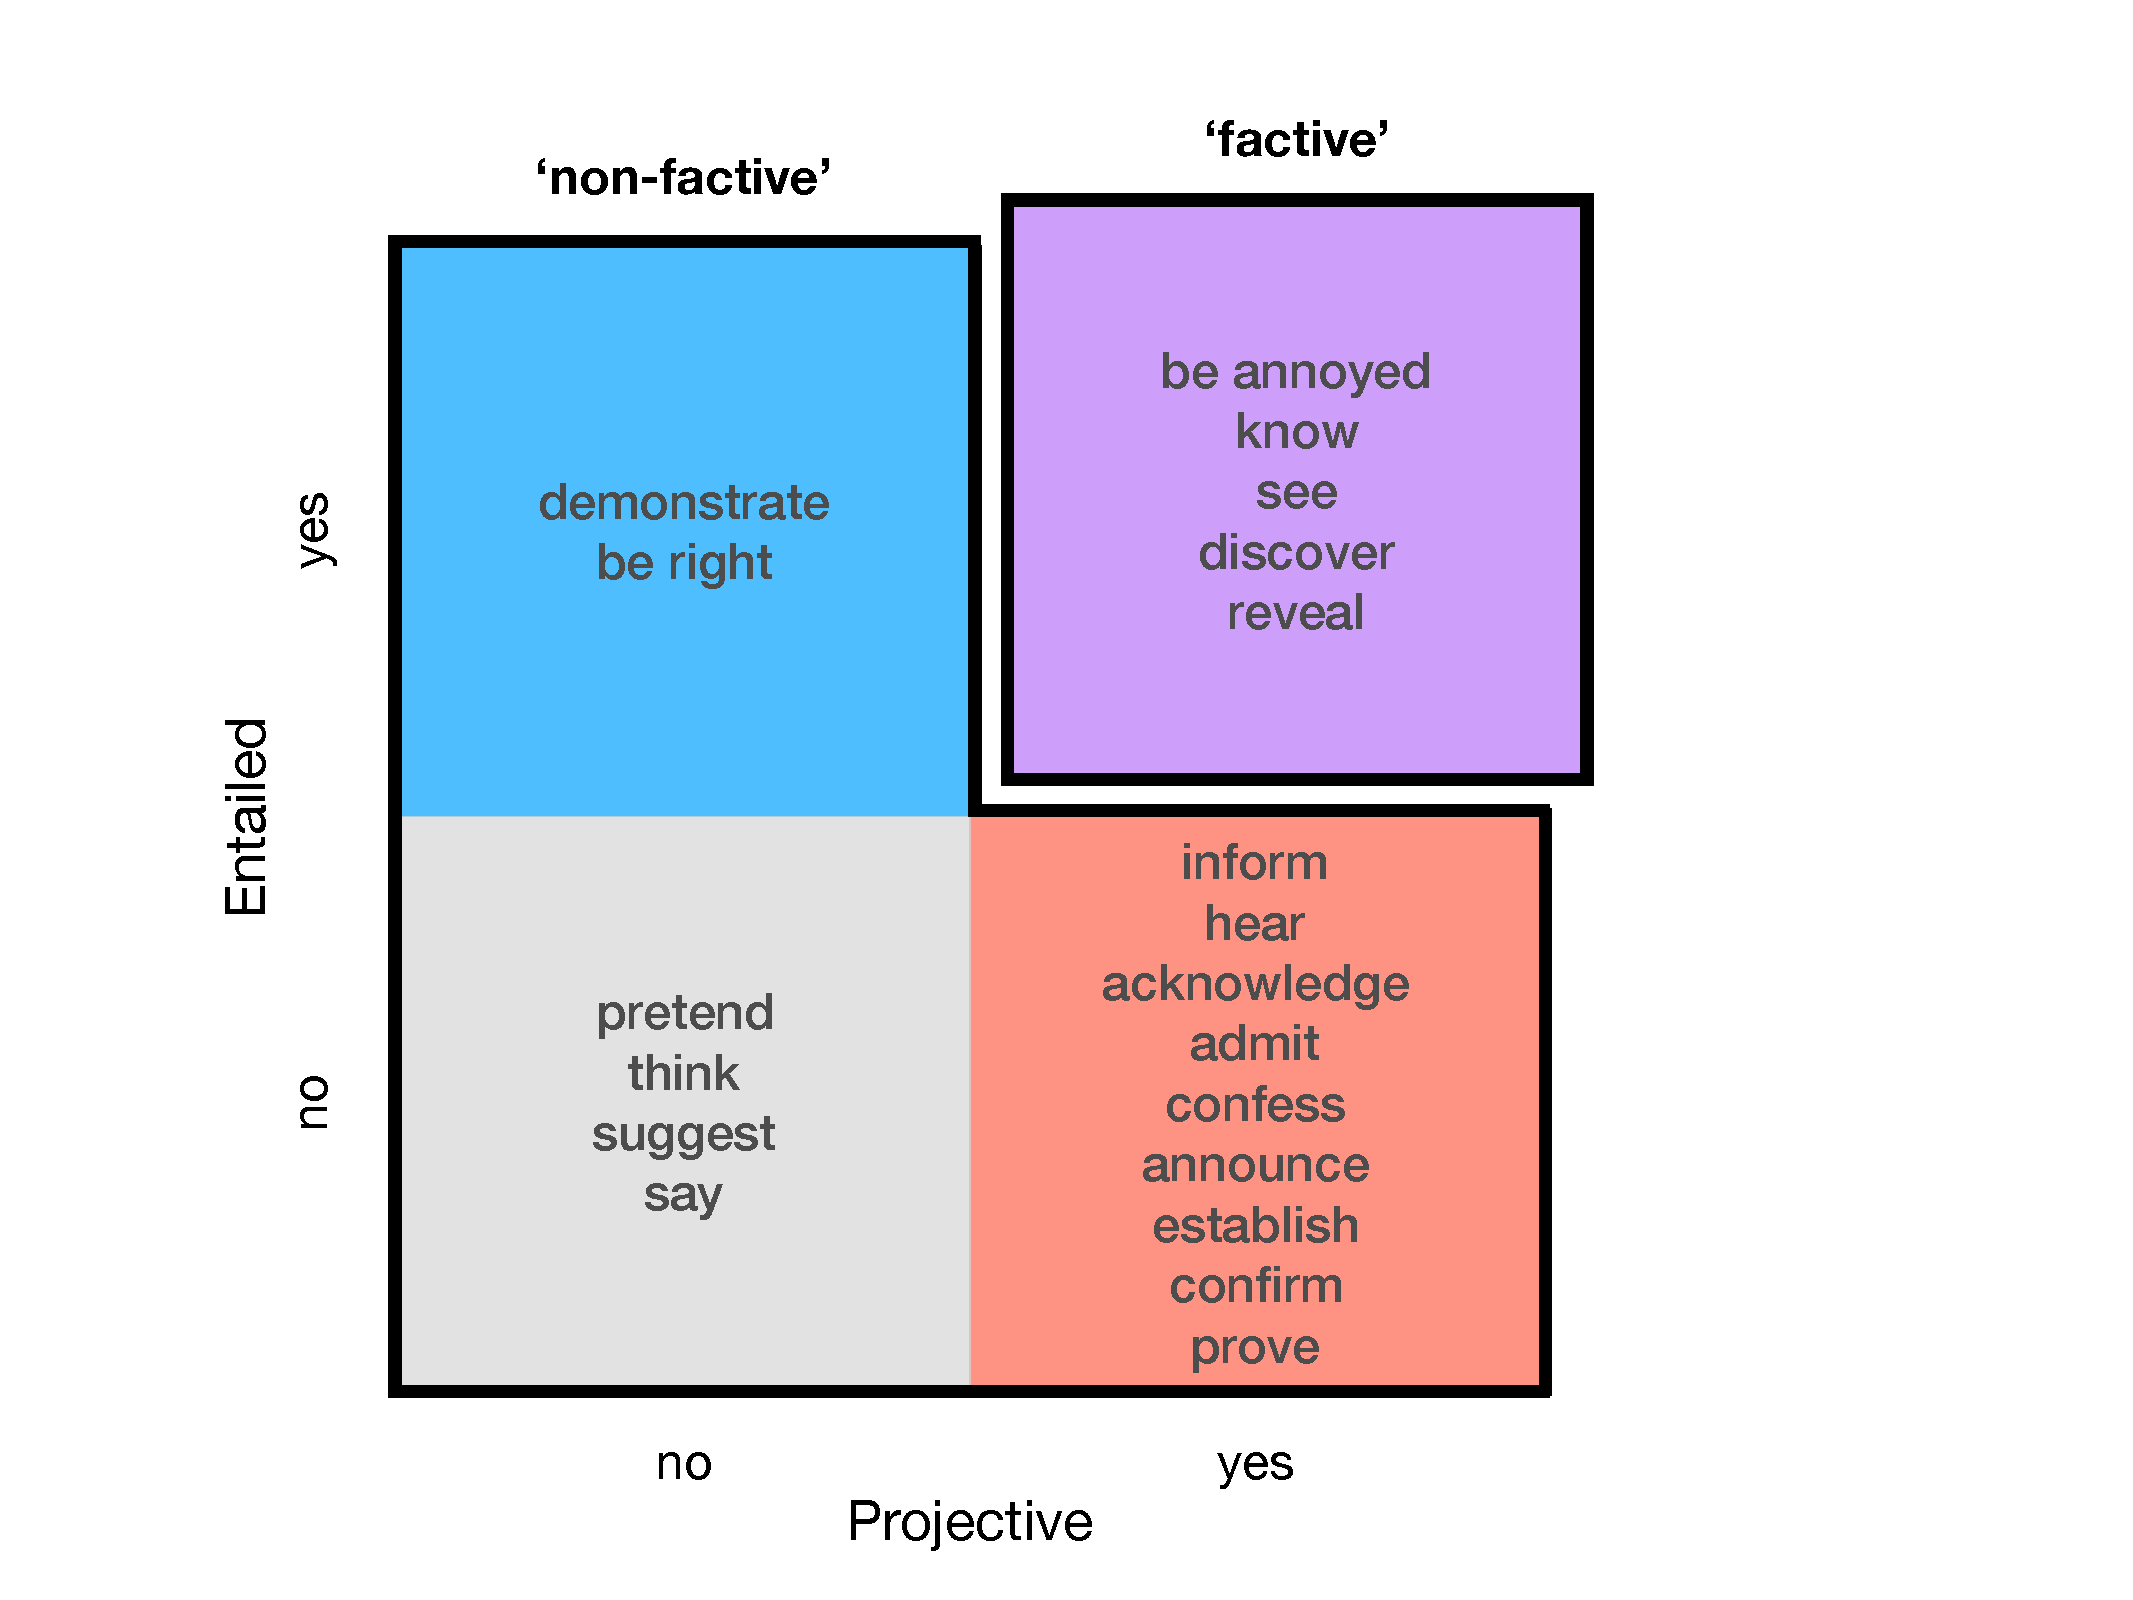
\includegraphics[trim={3.5cm 1cm 7cm 2cm},clip,width=.27\paperwidth]{../paper/figures/categorization}
%  \caption{Standard classification of 20 English predicates}\label{f-cat}
%\end{wrapfigure} 

\noindent
Projection analyses have largely limited their attention to `factive' predicates, like {\em know}, to the exclusion of `non-factive' ones, like {\em think}  (e.g., \cite{heim83,vds92,abrusan2011,abrusan2016,romoli2015} and \cite{best-question}). This limitation is motivated by the long-standing and widely-assumed assumption that `factive' predicates are empirically distinct from `non-factive' ones (see, e.g., \cite{karttunen71b,kiparsky-kiparsky71} and much literature thereafter): the content of the complement of a `factive' predicate is taken to be both projective and entailed, whereas it is not both projective and entailed for a `non-factive' one (e.g., \cite{gazdar79a}, \cite{ccmg90}, \cite{vds92},  \cite{schlenker10}, \cite{anand-hacquard2014}, \cite{spector-egre2015}). 

Despite the importance of the distinction between `factive' and `non-factive' predicates, the distinction has not been systematically investigated. Filling this lacuna is particularly pressing given that there is disagreement about which predicates are `factive'. For instance, \cite{schlenker10} assumed that {\em inform} is `factive', in contrast to \cite{anand-hacquard2014} who argued that the content of its complement is not entailed. Similarly, emotive predicates like {\em be annoyed} are taken to be `factive' by some (e.g., \cite{gazdar79a,abrusan2011,anand-hacquard2014}) but not others (e.g., \cite{klein1975,giannakidou1998,schlenker2003,egre2008}). We present the findings of experiments designed to investigate the distinction by measuring projectivity and entailment for 20 predicates; left panel of Fig.\ \ref{f-summary-categorical}. {\bf maybe add question marks in the figure after the predicates where people have disagreements? be annoyed, inform, establish, hear)}

{\bf Exp.~1:} Projectivity was measured with the `certain that' diagnostic: following \cite*{tbd-variability}, we assume that projectivity is a gradient property of utterance content. 

{\bf Exp.~2:} For entailment, we applied the `inference' diagnostic: $p$ entails $q$ iff $q$ follows from the truth of $p$; under the `contradictoriness' diagnostic, $p$ entails $q$ iff $p$ {\em but not} $q$ is contradictory. 

{\bf Results and discussion:} As shown in the right panel of Fig.\ \ref{f-summary-categorical}, the content of the complement of `factive' predicates (in purple) is entailed and highly projective whereas that of classical `non-factive' predicates (in grey) is not entailed and at most weakly projective, in line with intuitions reported in the literature. However, because projectivity is again observed to be a gradient property

\begin{wrapfigure}{r}{.77\textwidth}
\begin{subfigure}{.35\textwidth}
\centering
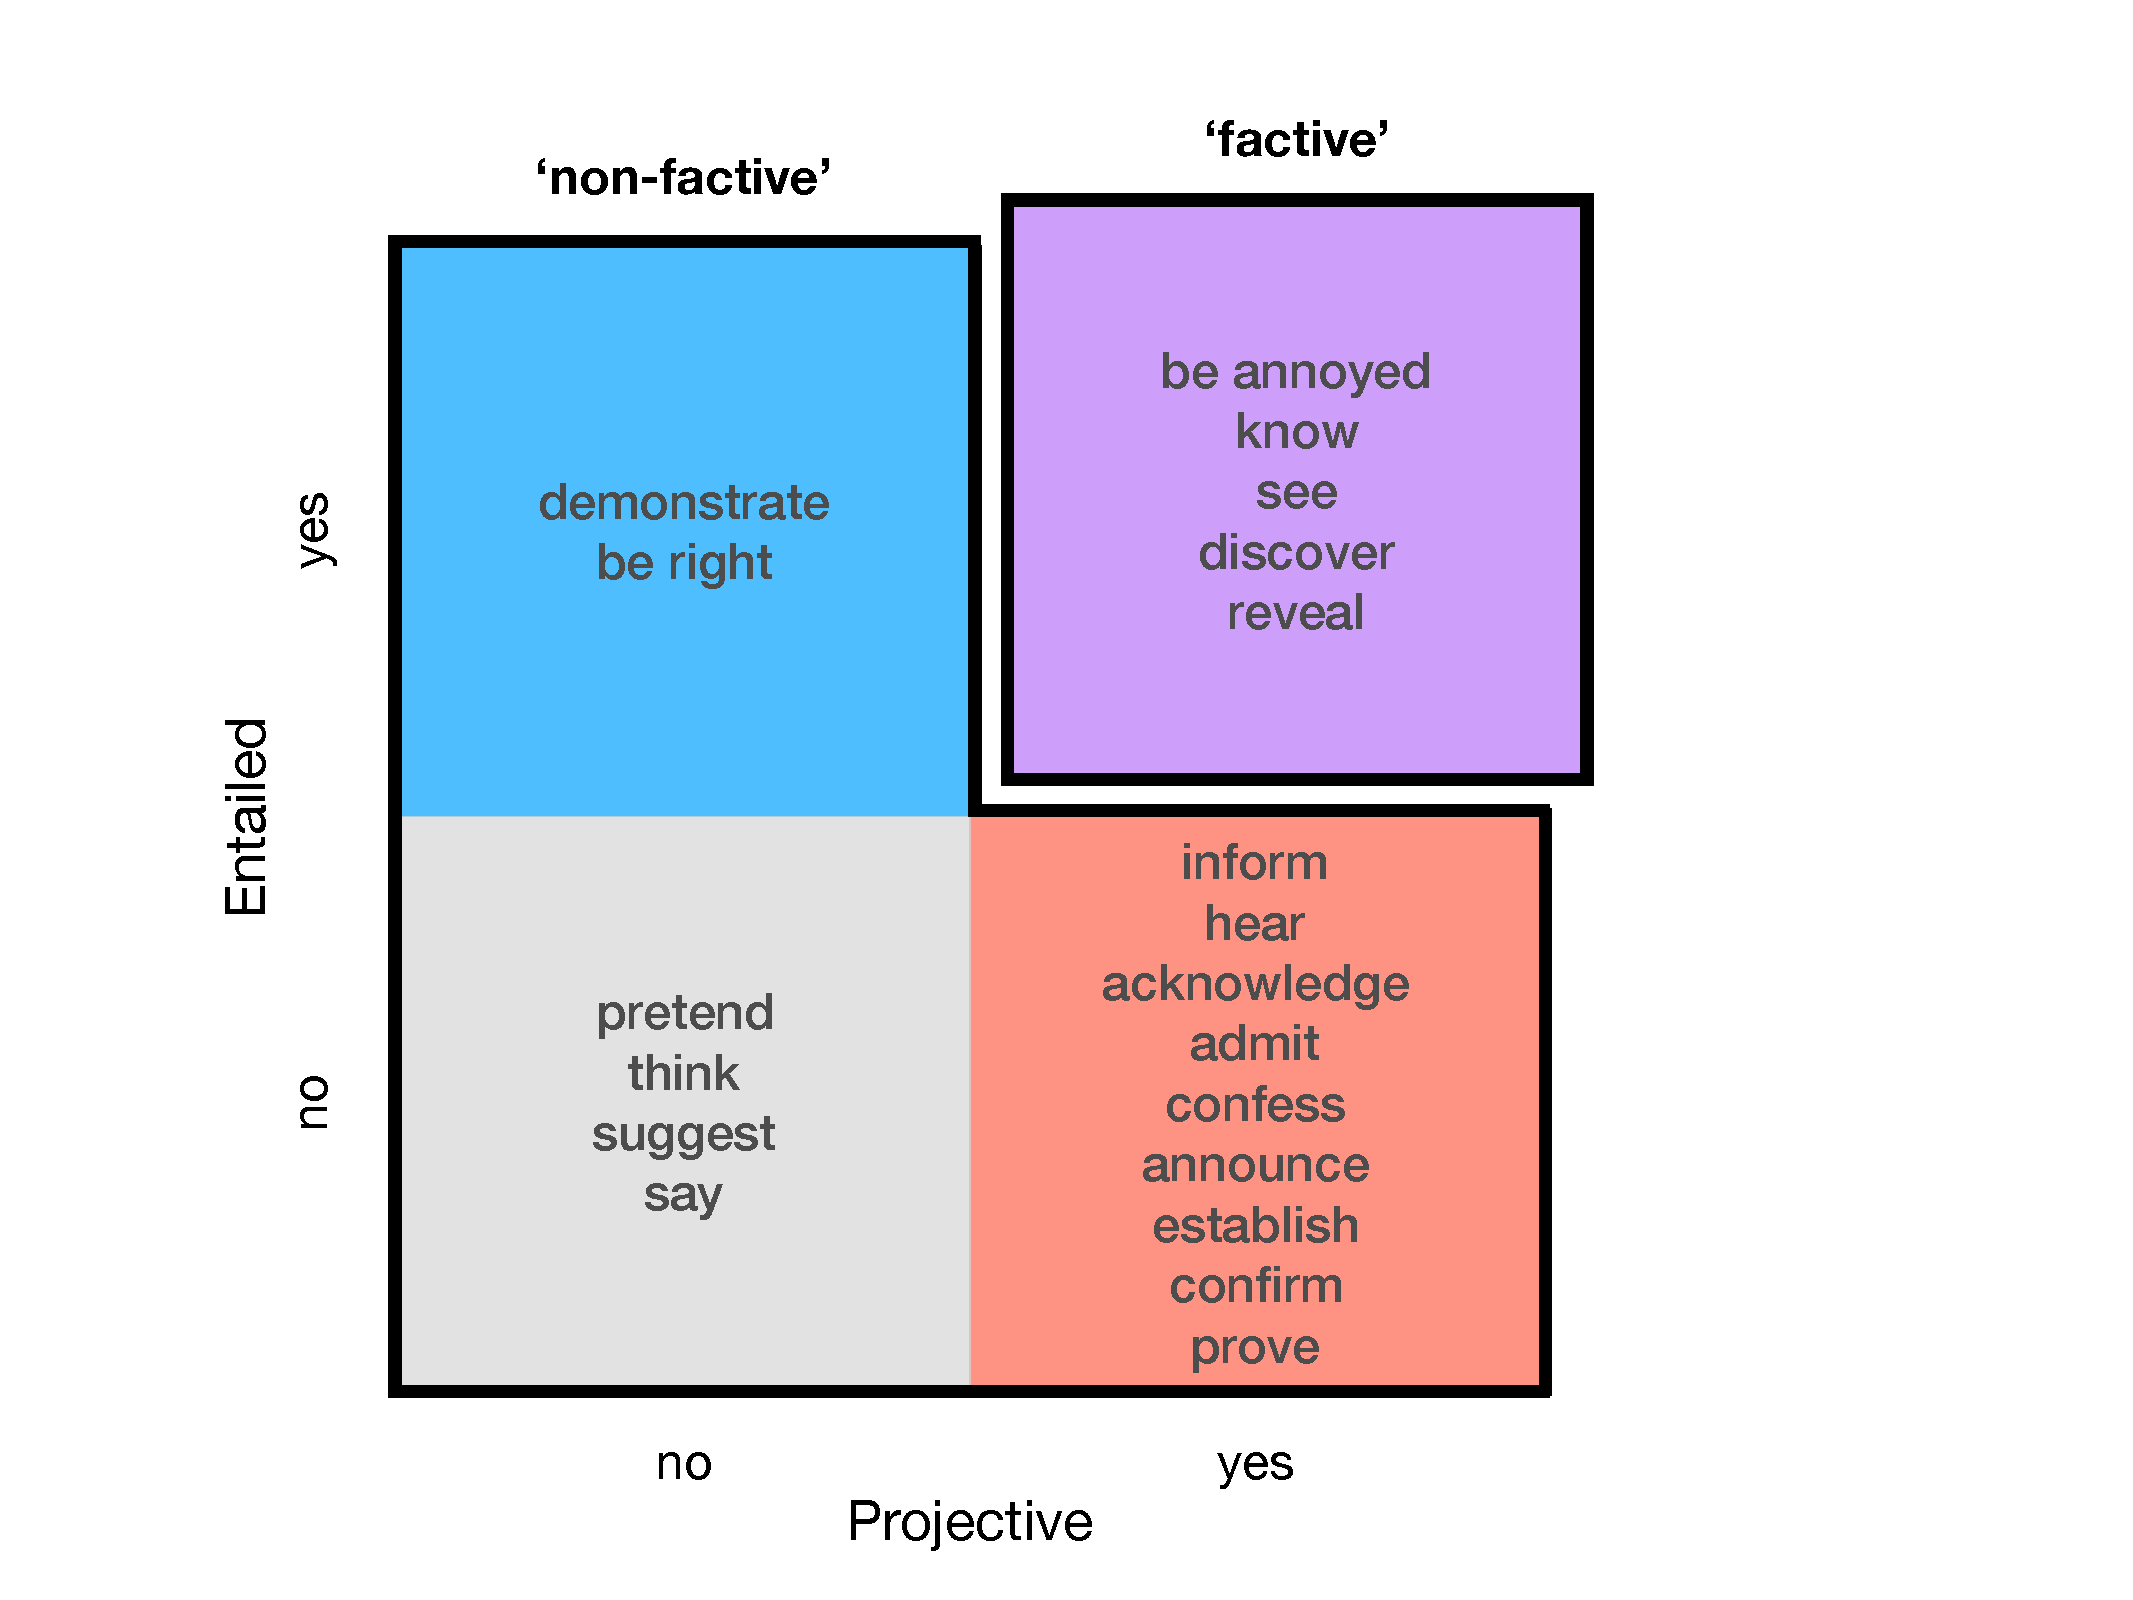
\includegraphics[trim={3.5cm 1cm 7cm 2cm},clip,width=.27\paperwidth]{../paper/figures/categorization}
%\caption{Assumed categorical classification}
\end{subfigure} %
\begin{subfigure}{.3\textwidth}
\centering
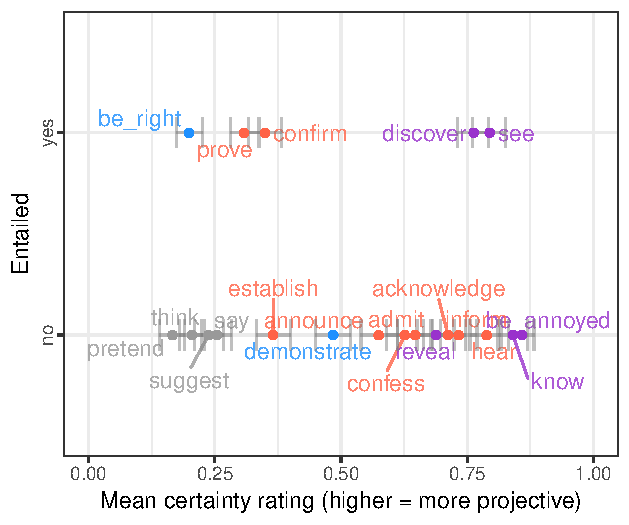
\includegraphics[width=.3\paperwidth]{../results/5-projectivity-no-fact/graphs/projection-by-inferenceEntailment}
%\caption{Experiment findings}
\end{subfigure}

\caption{20 English predicates: assumed categorical classification (left panel) vs.\ experiment findings (right panel; mean certainty rating with 95\% CIs, inference diagnostic for entailment.}\label{f-summary-categorical}

\end{wrapfigure}

\noindent
of utterance content (see also \cite{tbd-variability}), there is no non-arbitrary binary division of predicates by projectivity, thereby challenging the assumed categorical distinction between `factive' and `non-factive' predicates. The finding that the content of the complement of many `non-factive' predicates is projective constitutes an exciting challenge for future projection analyses.

{\bf (20\% mis-classified on Exp 2a, 6/20 on Exp 2b)}

{\bf somehow mention second entailment diagnostic} research on entailment needs to take the pragmatics of entailment judgments more seriously (see also \cite{demarneffe-etal2012}). 



%\begin{figure}[h]
%
%\begin{subfigure}{.35\textwidth}
%\centering
%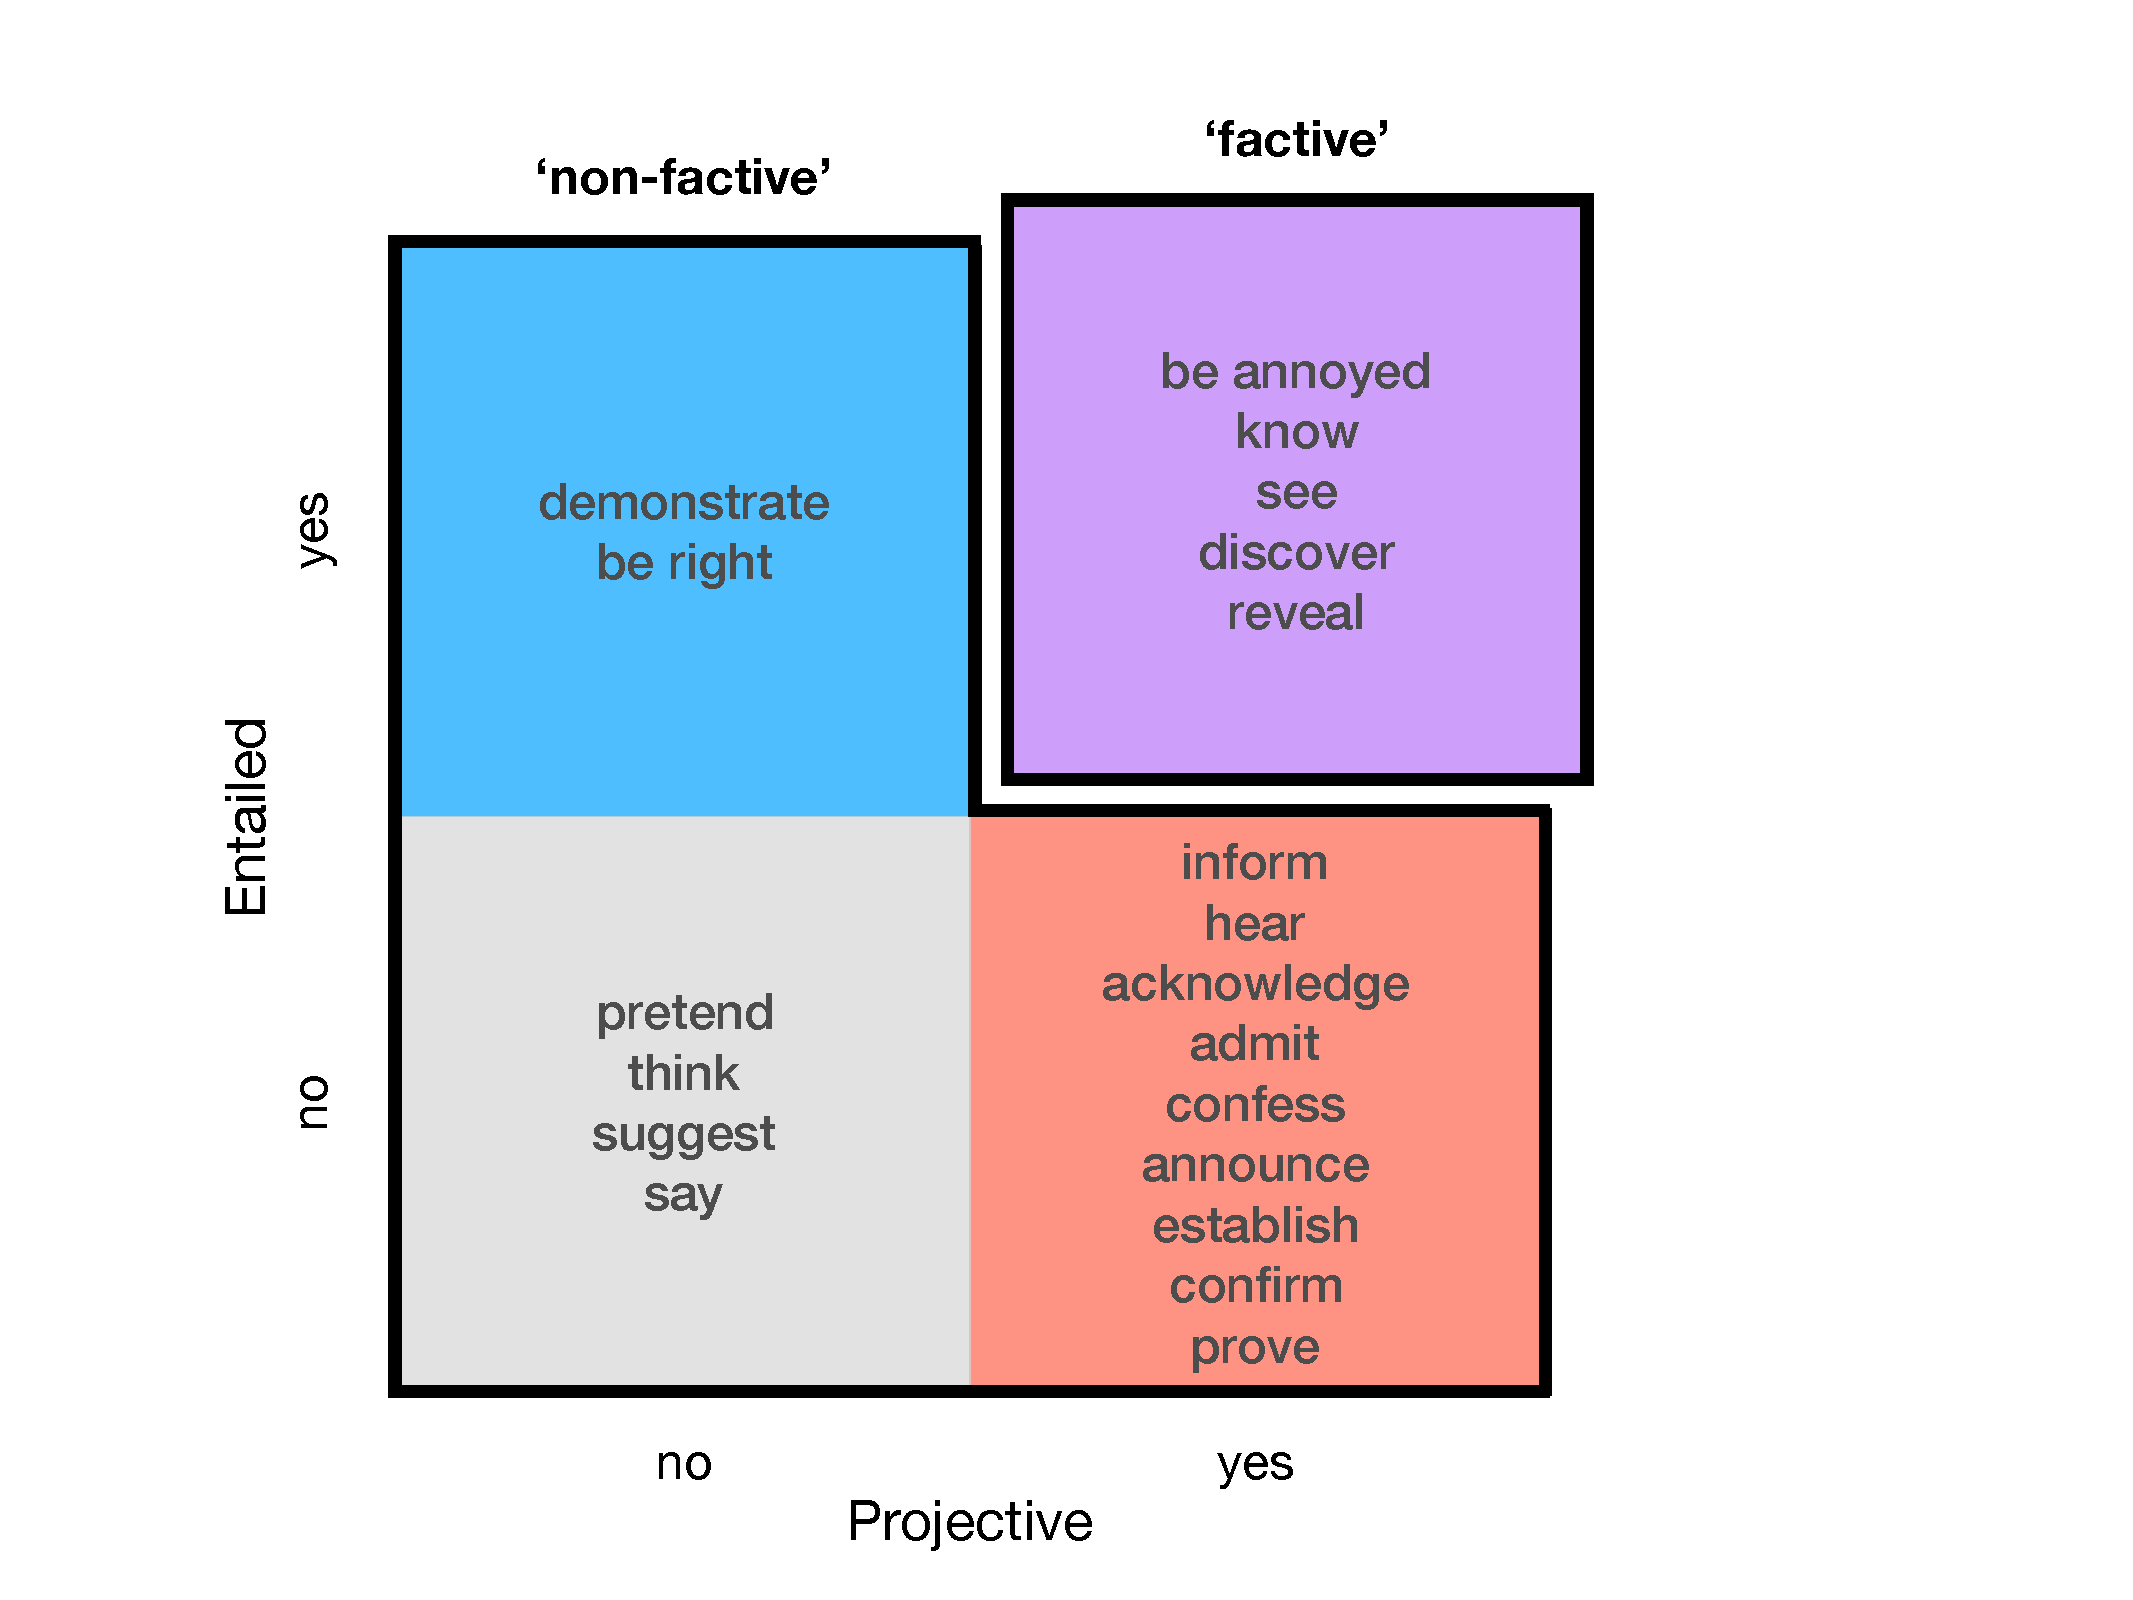
\includegraphics[trim={3.5cm 1cm 7cm 2cm},clip,width=.27\paperwidth]{../paper/figures/categorization}
%%\caption{Assumed categorical classification}
%\end{subfigure} %
%\begin{subfigure}{.3\textwidth}
%\centering
%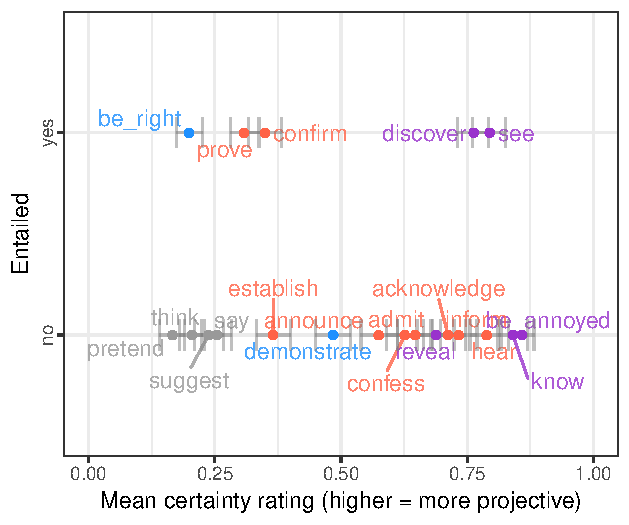
\includegraphics[width=.3\paperwidth]{../results/5-projectivity-no-fact/graphs/projection-by-inferenceEntailment}
%%\caption{Experiment findings}
%\end{subfigure}
%
%\caption{20 English predicates: assumed categorical classification (left panel) vs.\ experiment findings (right panel; mean certainty rating with 95\% CIs, inference diagnostic for entailment.}\label{f-summary-categorical}
%
%\end{figure}

\newpage

\bibliography{../bibliography}

\end{document}
